% pgfplots oracle fixture (hand-written): the options of the tikzpicture
% around an axis (behaviour AC1). The line width is reset when the axis
% begins; the colour reaches the box, embedded TikZ and all text, the font
% all text; the cycle list, grid and ticks keep their own colours.
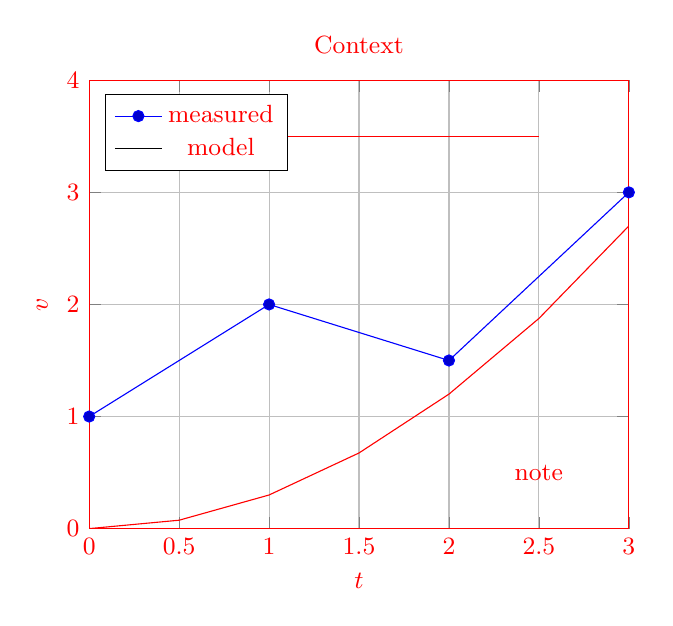
\begin{tikzpicture}[thick, font=\small, red]
\begin{axis}[xmin=0, xmax=3, ymin=0, ymax=4, grid=major, title={Context}, xlabel=$t$, ylabel=$v$, legend pos=north west]
\addplot coordinates {(0,1) (1,2) (2,1.5) (3,3)};
\addlegendentry{measured}
\addplot[domain=0:3, samples=7] {0.3*x^2};
\addlegendentry{model}
\draw (axis cs:0.5,3.5) -- (axis cs:2.5,3.5);
\node at (axis cs:2.5,0.5) {note};
\end{axis}
\end{tikzpicture}
